\section{Evidence production bổ sung và kế hoạch phục hồi}
\label{sec:production-evidence}
Các ảnh Render do người dùng cung cấp, đã đọc trực tiếp ngày 13/11/2026.
Capture time của ảnh chưa có; giờ event/deployed được giữ như hiển thị.
Đây là evidence deployment ngày13/11, độc lập với các HTTP snapshot sau đó.
Audit14/11 lúc10:31 UTC không cung cấp process SHA cho từng request; không
gán source của ảnh Render cho mọi GET mới (xem mục\ref{sec:deployment-release-delivery}).
Bản raw có credential/IP không đưa vào repository hoặc PDF. Các bản sao dùng
opaque redaction cục bộ đã mở kiểm tra lại; không dùng ảnh để suy ra secret/config
thực của backend. Full SHA source02452f2 được Git/GitHub xác nhận là
\path{02452f228712c3501c8d27f0f1ae737ad206785d}.

\begin{figure}[htbp]
\centering
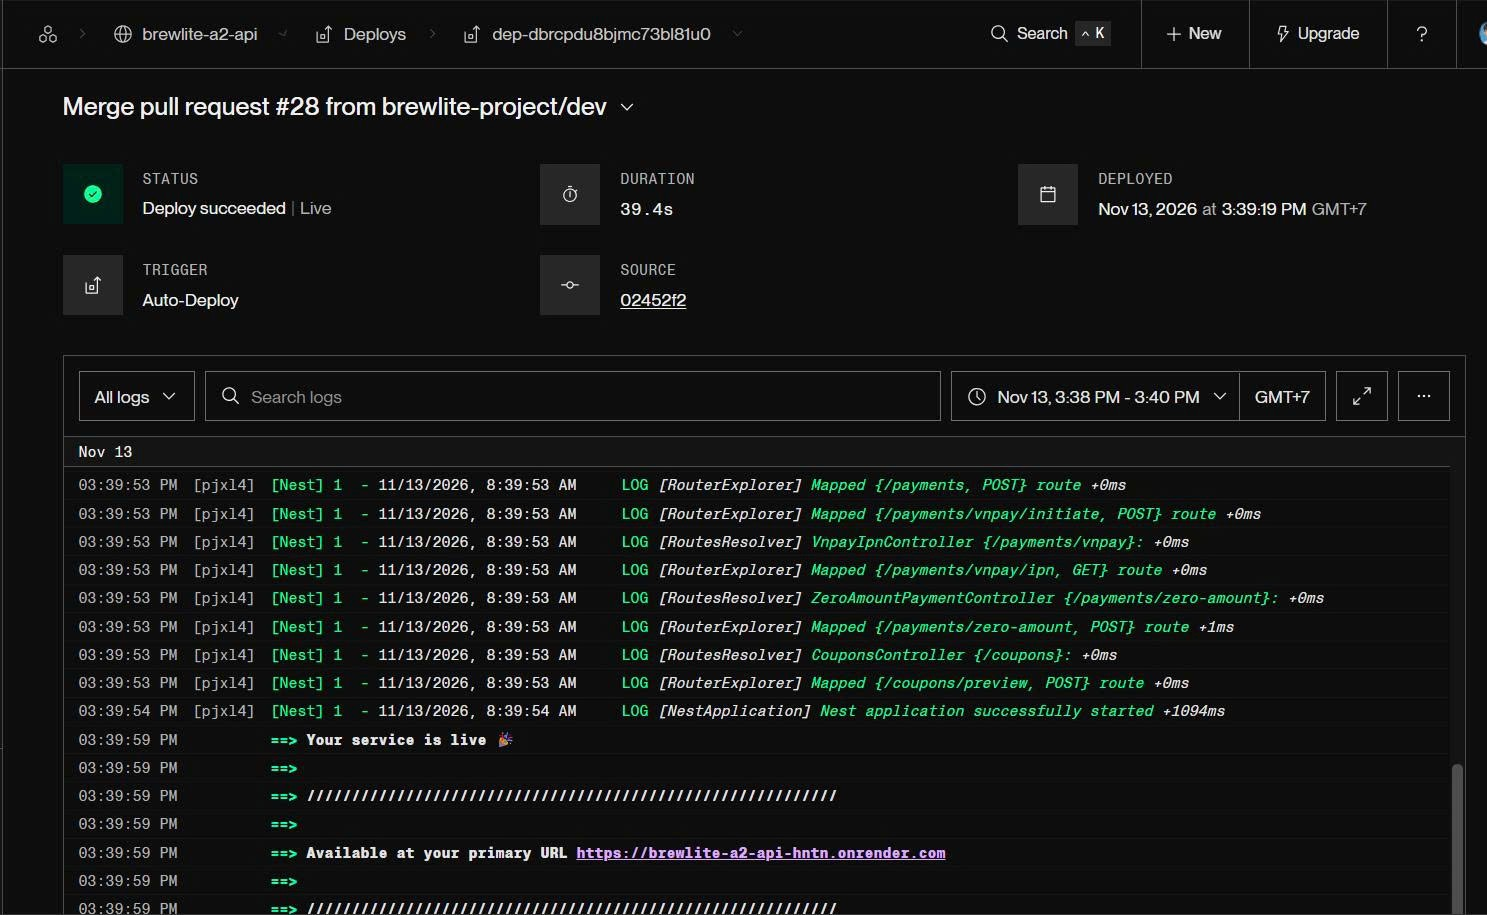
\includegraphics[width=\linewidth]{docs/delivery/evidence/render-deploy-02452f2.png}
\caption[Render Auto-Deploy Live02452f2]{Render Auto-Deploy succeeded/Live, source02452f2. Deployed field
13/11/2026 15:39:19 GMT+7 (08:39:19Z); Nest started15:39:54 và service live15:39:59.
Đây là deployment evidence, không phải timestamp của HTTP smoke.}
\label{fig:render-live-evidence}
\end{figure}

\clearpage
\begin{figure}[htbp]
\centering
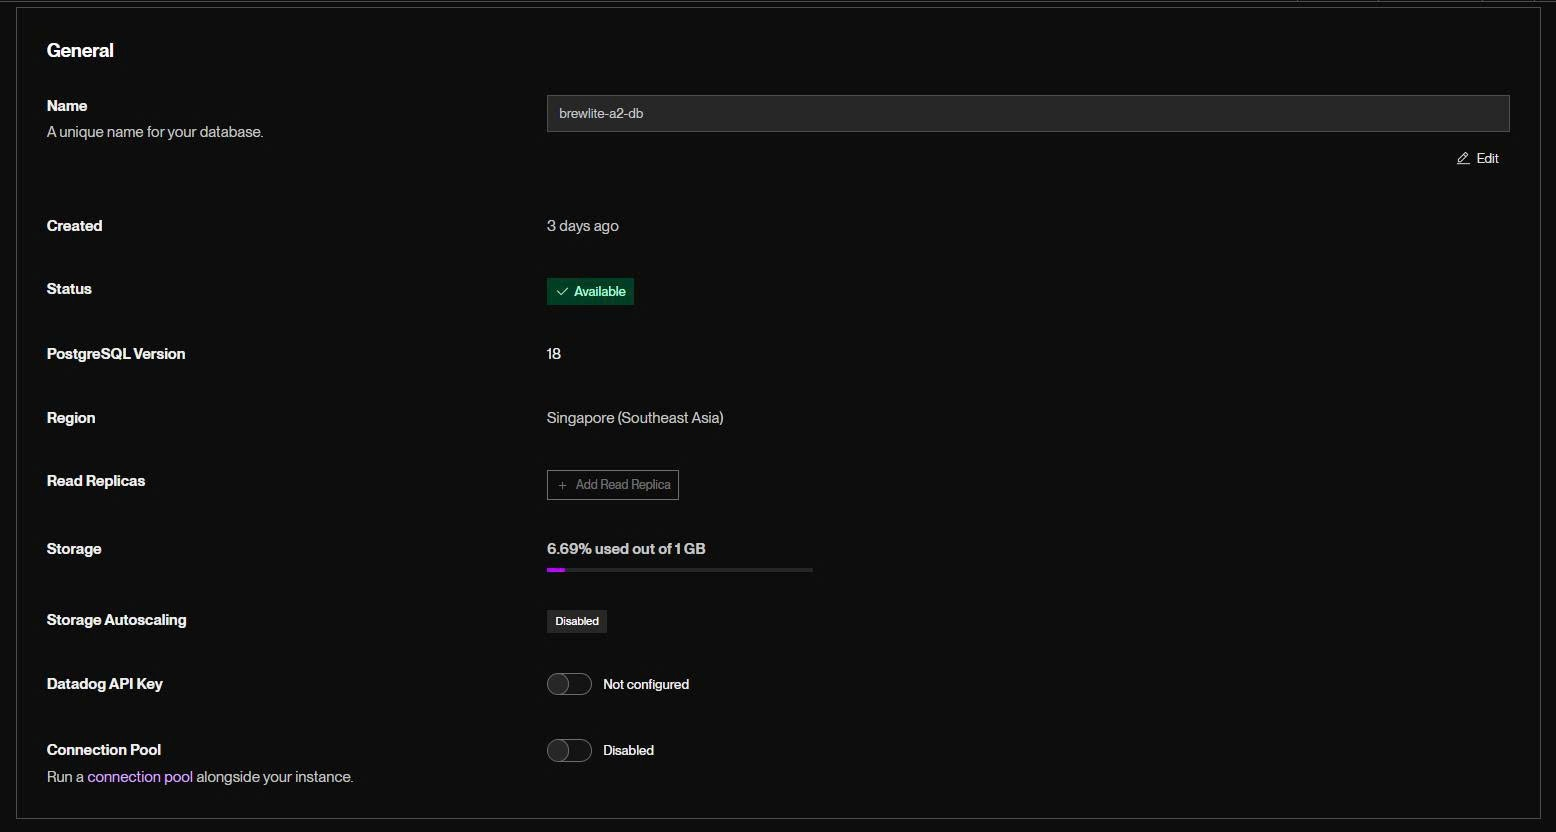
\includegraphics[width=\linewidth,height=0.55\textheight,keepaspectratio]{docs/delivery/evidence/render-db-plan.png}
\caption[Render PostgreSQL18 Free tại Singapore]{DB Available, PostgreSQL18, Singapore, Free1GB. Backend web tier và
Vercel plan vẫn chưa xác nhận; không suy từ tier database.}
\label{fig:render-db-plan-evidence}
\end{figure}
DB hết hạn \textbf{10/12/2026 theo dashboard}, xem ảnh expiry đã che trong
\path{docs/delivery/evidence/render-db-expiry-redacted.png}. Trước mốc đó nhóm
phải chọn nâng tier hoặc export/restore/migrate tới đích phù hợp. Chưa có người
vận hành/tiếp nhận, lịch backup/retention hoặc RPO/RTO được chốt. Không dùng grace
sau expiry làm thời gian đảm bảo demo. Free không có managed backup/PITR;
runbook mới chuẩn bị không được ghi là backup đã có hoặc restore verified.

\clearpage
\begin{figure}[htbp]
\centering
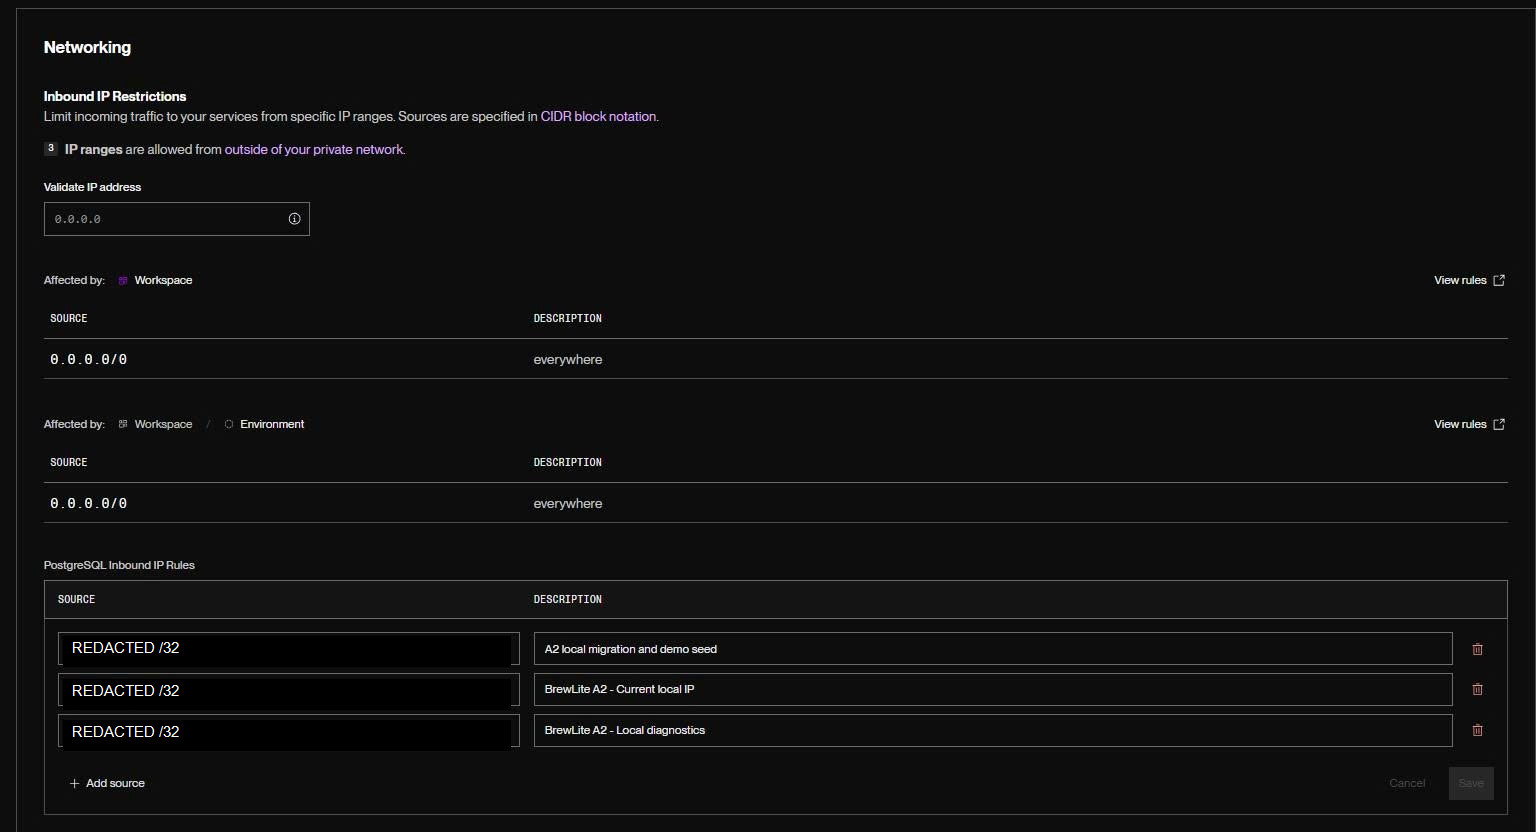
\includegraphics[width=\linewidth,height=0.62\textheight,keepaspectratio]{docs/delivery/evidence/render-db-network-redacted.png}
\caption[Render database external allowlist đã che IP]{Networking: workspace/environment allow-all và ba DB /32 đã che IP.
Theo Render inbound rules, traffic external phải được mọi cấp áp dụng cho phép;
DB đang restricted external, chưa private-only.}
\label{fig:render-db-network-evidence}
\end{figure}
AC3 cần manager xác nhận rule đã lưu, chủ/mục đích/thời hạn và quyết định liệu
admin external có hạn được chấp nhận hay phải private-only. Internal field
trong dashboard không chứng minh DATABASE\_URL thực của app; xác nhận bằng
mode/target-match/region association không có credential. Không đổi network
policy, environment hoặc kết nối DB trong lượt tài liệu này.

\subsection{Backup/restore và rollback có điều kiện}
Tools pg\_dump/pg\_restore18.6 đã có; chỉ chạy version check. Runbook tại
\path{docs/deployment.md}, mục11.5, dùng custom-format archive ở kho mã hóa
ngoài repo, PG* và PGPASSFILE qua secret manager/user-only ACL, TLS phù hợp
provider; không đặt credential trong lệnh/log. Kiểm tra TOC/hash chỉ là archive
check, không thay restore test. Không backup production trong lượt này.

Restore cần DB PostgreSQL18 mới rỗng/cô lập, manager xác nhận host/port/user/DB
khác production trước lệnh. Không dùng clean/drop hoặc ghi đè DB đang phục vụ.
Đối chiếu migrations/seed marker/constraints/counts và financial invariants;
cô lập scheduler/gateway callbacks, không seed Apply. Sau actual restore/test,
reviewer mới xác nhận usable backup. Cutover cần approval riêng và chấp nhận
khoảng mất dữ liệu, không tự sửa environment hoặc redeploy.

Candidate backend cũ2216b7a được PR26 báo Render Live/Sandbox payment success;
chưa có deployID/artifact retention hoặc approval làm rollback target.
Candidate này đã chứa migration10 additive seed\_executions. Giữ table/marker
và migration history khi rollback app; không xóa marker để ép seed. DB restore
trước10 có thể mất mọi ghi sau snapshot, không là rollback mặc định.
Frontend Preview2216b7a không chứng minh từng production domain, chưa eligible;
manager cần chọn target cũ phù hợp plan/schema/API/env/proxy.
Sau rollback được phép phải ghi UTC/IDs/SHA, health/catalog/migration state,
financial consistency/scheduler và smoke actual. Chưa thực hiện rehearsal.
